% MIL-STD-1553
% esquema del bus
% version 2021

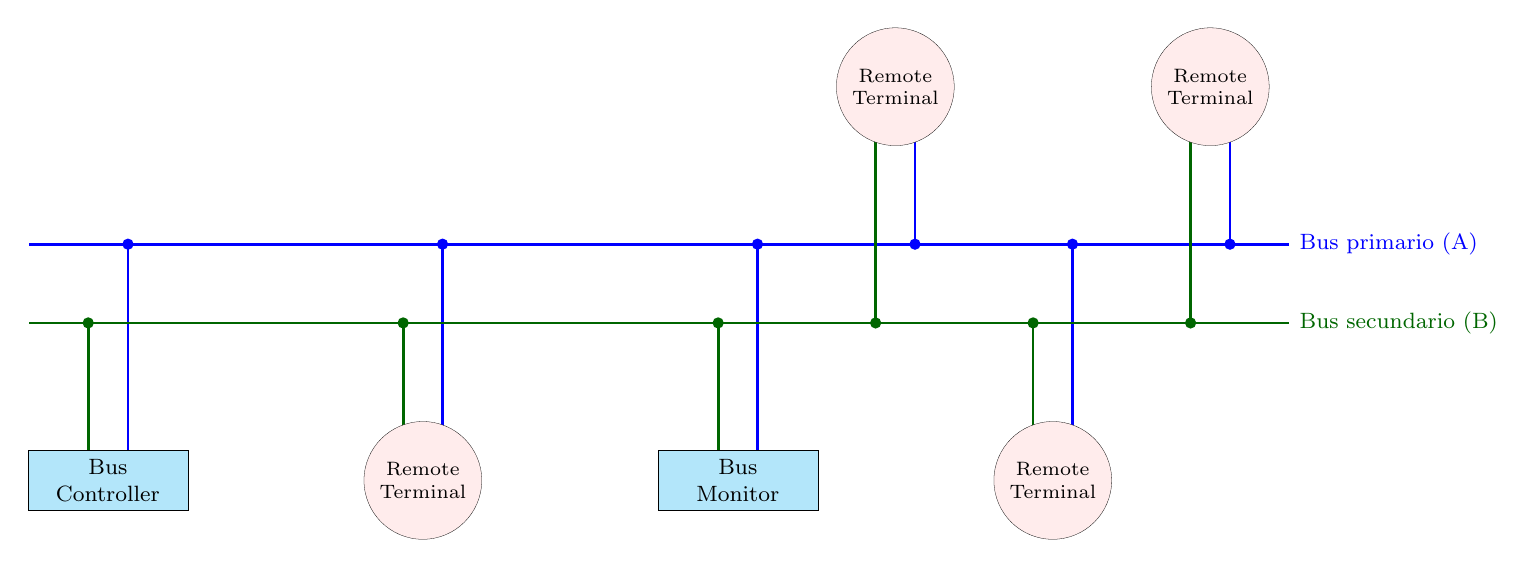
\begin{tikzpicture}[ node distance=1cm,
             conexion/.style = { circle, 
                                                 minimum size = 3 ,
                                              draw,
												fill ,
											inner sep=0 ,
                                                },
				font = \footnotesize , 
               Transmisor/.style ={ fill=cyan!30 , 
                          draw,
                          line width= 0.1 , 
						text width=1.8cm,
						align = center
                        } ,
               Receptor/.style ={  font = \scriptsize, 
						circle ,
                          fill=pink!30 , 
                          draw,
%						text width=1.2cm,
						align = center ,
                          line width= 0.1 , 
                        } ,
                     ]

% grilla
%  \draw[ green!50!black] (0,0) grid (20,10) ;

% Bus primario
\draw[line width=1, blue]  (0 , 4) -- +(16 , 0) node[above, right] {Bus primario (A)}
                       (1.255 , 4 ) node[conexion ] {} -- +(0 , -3) 
                       (5.25 , 4 ) node[conexion ] {} -- +(0 , -3) 
                       (9.25 , 4 ) node[conexion ] {} -- +(0 , -3)
                        (11.25 , 4 ) node[conexion ] {} -- +(0 , 2)
                       (13.25 , 4 ) node[conexion ] {} -- +(0 , -3) 
                       (15.25 , 4 ) node[conexion ] {} -- +(0 , 2) 
;

% Bus secundario
\draw[line width=1, green!40!black]  (0 , 3) -- +(16 , 0) node[above, right] {Bus secundario (B)} 
                       (0.75 , 3 ) node[conexion ] {} -- +(0 , -2) 
                       (4.75 , 3 ) node[conexion ] {} -- +(0 , -2) 
                       (8.75 , 3 ) node[conexion ] {} -- +(0 , -2) 
                      (10.75 , 3 ) node[conexion ] {} -- +(0 ,  3)
                      (12.75 , 3 ) node[conexion ] {} -- +(0 ,  -2)
                      (14.75 , 3 ) node[conexion ] {} -- +(0 ,  3)
;

% Elementos del bus
\draw ( 1 ,1 ) node[Transmisor] (BS) {Bus \\Controller} 
            +( 4 , 0 ) node[Receptor] (RT1) {Remote \\Terminal} 
            +( 8 , 0 ) node[Transmisor] (BM) {Bus \\ Monitor} 
            +( 10 , 5 ) node[Receptor] (RT2) {Remote \\Terminal} 
            +( 12 , 0 ) node[Receptor] (RT3) {Remote \\Terminal} 
            +( 14 , 5 ) node[Receptor] (RT4) {Remote \\Terminal} 
;





\end{tikzpicture}